% L5a student companion deck.
%
% The frame order mirrors the lecture notebook so students can take notes while
% the instructor works through the notebook. The disclaimer is intentionally
% slide 2, by instructor preference.
\documentclass[aspectratio=169,11pt]{beamer}
\usepackage{vnslides}

\newcommand{\Pmeasure}{\mathbb{P}}
\newcommand{\E}{\mathbb{E}}
\newcommand{\Var}{\operatorname{Var}}
\newcommand{\Cov}{\operatorname{Cov}}
\newcommand{\gbar}{\bar g}
\newcommand{\bA}{\mathbf{A}}
\newcommand{\bC}{\mathbf{C}}
\newcommand{\bG}{\mathbf{G}}
\newcommand{\bZ}{\mathbf{Z}}
\newcommand{\bw}{\mathbf{w}}
\newcommand{\bg}{\mathbf{g}}
\newcommand{\Sg}{\hat{\boldsymbol{\Sigma}}_{g}}
\newcommand{\Ch}{\hat{\mathbf{C}}}

\title{\texorpdfstring{{\vnheavy L5a}}{L5a}: Multiple Asset Geometric Brownian Motion}
\subtitle{CHEME 5660 Cornell University}
\author{Copyright Jeffrey Varner 2026. All Rights Reserved}

\begin{document}

\vntitlepage

\begin{frame}{Disclaimer and Risks}
  \vspace{0.6em}
  \textbf{\ink{Training only.}} This content is for training and informational
  purposes only. The teaching team does not make, give, or endorse any offer or
  solicitation to buy or sell securities or derivative products, or provide
  investment or trading advice or strategy.

  \vspace{1.1em}
  \textbf{\ink{Risk.}} Trading involves risk and is generally not recommended for
  those with limited resources, experience, or a low risk tolerance. Past
  performance does not guarantee future success.

  \vspace{1.1em}
  \textbf{\ink{Responsibility.}} You are responsible for your investment decisions
  based on your financial circumstances, objectives, risk tolerance, and
  liquidity needs.
\end{frame}

\begin{frame}{Objectives for Today}
By the end of this lecture, you will be able to:

  \vspace{0.8em}
  \begin{itemize}\setlength{\itemsep}{0.8em}
    \item \hilite{Model assets that move together}: extend geometric
      Brownian motion (GBM) from one asset to several and explain how
      covariance captures their shared fluctuations.
    \item \hilite{Interpret covariance from data}: explain what historical
      growth rates tell us about individual asset variability and how
      assets move together.
    \item \hilite{Connect investment weights to portfolio wealth}: explain
      how allocations shape portfolio outcomes and use the Dirichlet
      distribution to explore different investment mixes.
  \end{itemize}
\end{frame}

\begin{frame}{Lectures and Examples}
\textbf{\ink{Lecture:}}
  \href{https://github.com/varnerlab/CHEME-5660-CourseRepository-Fall-2026/blob/main/lectures/week-5/L5a/CHEME-5660-L5a-Lecture-MultipleAsset-GBM-Fall-2026.ipynb}{Multiple Asset Geometric Brownian Motion}

  \vspace{0.7em}
  \textbf{\ink{Example:}}
  \href{https://github.com/varnerlab/CHEME-5660-CourseRepository-Fall-2026/blob/main/lectures/week-5/L5a/CHEME-5660-L5a-Example-OOS-SAGBM-Fall-2026.ipynb}{Out-of-Sample Price Predictions}

  How well does a model fitted to 2014--2024 data describe future prices?
  We compare its prediction bands with prices observed in 2025.

  \vspace{0.7em}
  \textbf{\ink{Example:}}
  \href{https://github.com/varnerlab/CHEME-5660-CourseRepository-Fall-2026/blob/main/lectures/week-5/L5a/CHEME-5660-L5a-Example-CovarianceMatrix-Fall-2026.ipynb}{Covariance and Correlation from Data}

  How do firms' growth rates move together? We estimate covariance and
  correlation from historical data and connect them to the price model.

  \vspace{0.7em}
  \textbf{\ink{Example:}}
  \href{https://github.com/varnerlab/CHEME-5660-CourseRepository-Fall-2026/blob/main/lectures/week-5/L5a/CHEME-5660-L5a-Example-Dirichlet-PortfolioWeights-Fall-2026.ipynb}{Portfolio Weights and the Dirichlet Distribution}

  How does the investment mix affect growth and risk? We explore portfolio
  weights with the Dirichlet distribution and follow buy-and-hold wealth.
\end{frame}

\begin{frame}{Concept Review: Single Asset GBM Model}
  Recall that geometric Brownian motion (GBM) describes share price changes
  through drift and random fluctuations, both proportional to the current price:
  \[
    \frac{dS(t)}{S(t)}
    =\underbrace{\mu\,dt}_{\text{drift}}
    +\underbrace{\sigma\,dW(t)}_{\text{random fluctuations}}.
  \]

  Here, $S(t)$ is the share price (dollars per share), with initial price
  $S(0)=S_0>0$, and $dW(t)$ is a Wiener-process increment.

  \vspace{0.6em}
  With time measured in years, the constant parameters are:
  \begin{itemize}\setlength{\itemsep}{0.65em}
    \item \hilite{Drift $\mu\in\mathbb R$}: the expected proportional price
      change per unit time (year$^{-1}$).
    \item \hilite{Volatility $\sigma>0$}: sets the size of the random
      fluctuations (year$^{-1/2}$).
  \end{itemize}
\end{frame}

\begin{frame}{Concept Review: Growth and Volatility}
  Over an observation interval $\Delta t>0$ years, the growth rate is:
  \[
    g_j=\frac{1}{\Delta t}\ln\!\left(\frac{S_{t_j}}{S_{t_{j-1}}}\right),
    \qquad t_j=j\Delta t.
  \]

  Under GBM, its mean and standard deviation are:
  \[
    \underbrace{\mu_g=\E[g_j]=\mu-\frac{\sigma^2}{2}}_{\text{mean growth rate}},
    \qquad
    \underbrace{\sqrt{\Var(g_j)}=\frac{\sigma}{\sqrt{\Delta t}}}_{\text{growth-rate standard deviation}}.
  \]
  Drift $\mu$ and mean growth rate $\mu_g$ both have units year$^{-1}$,
  but differ by $\sigma^2/2$.

  \vspace{0.5em}
  From the sample growth-rate standard deviation $\sigma_g$, we estimate
  volatility as:
  \[
    \hat\sigma=\sigma_g\sqrt{\Delta t}.
  \]
\end{frame}

\begin{frame}{Concept Review: The One-Step Transition}
  For a grid of $N$ steps, $t_j=j\Delta t$, the exact transition from L4b is:
  \[
    \boxed{S_{t_j}=S_{t_{j-1}}\exp\!\Bigl[\mu_g\Delta t+
      \sigma\sqrt{\Delta t}\,Z_j\Bigr],\qquad j=1,\ldots,N.}
  \]
  Here, $Z_1,\ldots,Z_N$ are independent standard normal draws, one per step.

  \vspace{0.7em}
  For a single horizon $T>0$, we can sample the terminal price directly:
  \[
    S_T=S_0\exp\!\Bigl[\mu_gT+\sigma\sqrt{T}\,Z\Bigr],
    \qquad Z\sim\mathcal N(0,1).
  \]

  \vspace{0.5em}
  Repeated one-step draws generate a price path. The fixed-horizon form
  samples the price at the selected time $T$.
\end{frame}

\begin{frame}{Example: Out-of-Sample Price Predictions}
\textbf{\ink{Example:}}
  \href{https://github.com/varnerlab/CHEME-5660-CourseRepository-Fall-2026/blob/main/lectures/week-5/L5a/CHEME-5660-L5a-Example-OOS-SAGBM-Fall-2026.ipynb}{Test predictions against later observations}

  \vspace{0.7em}
  How well does a model fitted to historical prices describe prices
  observed afterward?

  \vspace{0.5em}
  \begin{itemize}\setlength{\itemsep}{0.6em}
    \item Use the mean growth rate and volatility estimated from 2014--2024 data.
    \item Simulate prices for 2025 and compare prediction bands with
      observed prices.
    \item Measure the fraction of dates with observed prices inside each band,
      first for one firm and then across the dataset.
  \end{itemize}

  \slidenote{Next question:}{how can this price distribution tell us the probability of exceeding a target return at a scheduled sale?}
\end{frame}

\begin{frame}{Catch-up: The GBM Trade Rule}
  Suppose we buy $n_0>0$ shares at $S_0>0$ and sell them at $S_T$ after
  $T>0$ years. Assume no dividends or trading costs.

  \vspace{0.6em}
  Let $g_y$ be the constant, continuously compounded benchmark growth rate
  (year$^{-1}$).

  \vspace{0.6em}
  Dividing the net present value (NPV) by the initial investment gives
  the \hilite{scaled NPV}, our discounted fractional return:
  \[
    \rho_T=\frac{\operatorname{NPV}(g_y,T)}{n_0S_0}
    =\left(\frac{S_T}{S_0}\right)e^{-g_yT}-1.
  \]

  \vspace{0.4em}
  A positive $\rho_T$ means that discounted sale proceeds exceed
  the purchase cost. We use GBM to describe the uncertain sale price $S_T$.
\end{frame}

\begin{frame}{Catch-up: The Target Probability}
  For a target scaled NPV $\rho_\star>-1$, GBM gives the probability of
  exceeding the target at the scheduled sale time $T$:
  \[
    \boxed{\Pmeasure(\rho_T>\rho_\star)
    =1-\Phi\!\left(\frac{\ln(1+\rho_\star)+g_yT-\mu_gT}{\sigma\sqrt T}\right).}
  \]

  Here, $\mu_g$ is the mean growth rate, $\sigma>0$ is volatility, and
  $\Phi$ is the standard normal cumulative distribution function.

  \vspace{0.5em}
  The $\Phi$ term gives the probability of finishing at or below the target.
  Subtracting it from one gives the probability of exceeding the target.

  \vspace{0.5em}
  Next, we extend the price model to several correlated assets.

  \slidenote{L4b review:}{\href{https://github.com/varnerlab/CHEME-5660-CourseRepository-Fall-2026/blob/main/lectures/week-4/L4b/CHEME-5660-L4b-Lecture-SingleAsset-GeometricBrownianMotion-TradeRule-Fall-2026.ipynb}{GBM trade-rule derivation}\quad\href{https://github.com/varnerlab/CHEME-5660-CourseRepository-Fall-2026/blob/main/lectures/week-4/L4b/CHEME-5660-L4b-Example-GBM-NPV-TradeRule-Fall-2026.ipynb}{Terminal-target probability example}}
\end{frame}

\begin{frame}{Multiple Asset Geometric Brownian Motion}
  Independent GBM models assume zero covariance between assets' growth rates.
  Multiple asset geometric Brownian motion (MAGBM) allows correlated growth rates.

  \vspace{0.5em}
  For $M\ge2$ assets, let $g_i$ be asset $i$'s growth rate over the same
  interval $\Delta t>0$ years. The model uses a matrix
  $\bC\in\mathbb R^{M\times M}$ related to growth-rate covariance by:
  \[
    \underbrace{C_{ij}}_{\text{covariance rate}}
    =\Delta t\;\underbrace{\Cov(g_i,g_j)}_{\text{growth-rate covariance}}.
  \]

  Growth-rate covariance has units year$^{-2}$; multiplying by $\Delta t$
  gives $C_{ij}$ units of year$^{-1}$.

  \vspace{0.5em}
  The diagonal entries $C_{ii}=\sigma_i^2$ give squared volatilities.
  Off-diagonal entries have the same signs as the growth-rate covariances.
\end{frame}

\begin{frame}{Building Correlated Fluctuations}
  Start with increments $dW_1,\ldots,dW_M$ from independent standard
  Wiener processes.
  For two assets, the random terms in their price equations are:
  \[
    \begin{aligned}
      \text{Asset 1:}\qquad & A_{11}\,dW_1+A_{12}\,dW_2,\\[0.5em]
      \text{Asset 2:}\qquad & A_{21}\,dW_1+A_{22}\,dW_2.
    \end{aligned}
  \]

  Both assets use the same two random inputs. Their coefficients determine
  how strongly each asset responds to each input.

  \vspace{0.5em}
  Each row of the \hilite{loading matrix} $\bA$ contains one asset's
  coefficients. We choose $\bA$ to reproduce the covariance rate:
  \[
    \bA\bA^{\top}=\bC.
  \]
  For $M$ assets, $\bA$ is $M\times M$, with entries in year$^{-1/2}$.
\end{frame}

\begin{frame}{Multiple Asset GBM: The Price Model}
  Let $S_i(t)$ be asset $i$'s share price, with $S_i(0)>0$.
  For $i\in\mathcal P=\{1,\ldots,M\}$, the model is:
  \[
    \frac{dS_i(t)}{S_i(t)}
    =\underbrace{\mu_i\,dt}_{\text{drift}}
    +\underbrace{\textstyle\sum_{\ell=1}^{M}A_{i\ell}\,dW_\ell(t)}_{\text{random contribution to asset }i}.
  \]
  A \hilite{Wiener increment} $dW_\ell(t)$ is a normally distributed random
  change over $dt$, with mean zero and variance $dt$. Row $i$ of $\bA$
  combines these shared inputs.

  \vspace{0.5em}
  Drifts $\mu_i$ (year$^{-1}$) and $\bA$ remain constant, so
  $\bC=\bA\bA^{\top}$ is also constant.

  \vspace{0.5em}
  As in L4b, applying It\^o's lemma gives the mean growth rate:
  \[
    \mu_{g,i}=\mu_i-\frac{C_{ii}}{2}
    =\mu_i-\frac{\sigma_i^2}{2}.
  \]
\end{frame}

\begin{frame}{Why the \texorpdfstring{$\bA\bA^{\top}$}{AAT} Factorization?}
  Independent Wiener increments have covariance:
  \[
    \Cov(dW_\ell,dW_k)=
    \begin{cases}
      dt, & \ell=k,\\
      0, & \ell\ne k.
    \end{cases}
  \]
  Thus, only terms with matching indices contribute to the covariance
  of the random terms for assets $i$ and $j$:
  \[
    \begin{aligned}
      \Cov\!\left(\sum_{\ell=1}^{M}A_{i\ell}\,dW_\ell,\,
                  \sum_{k=1}^{M}A_{jk}\,dW_k\right)
      &=\sum_{\ell=1}^{M}A_{i\ell}A_{j\ell}\,dt\\[0.5em]
      &=(\bA\bA^{\top})_{ij}\,dt.
    \end{aligned}
  \]
  Choosing $\bA\bA^{\top}=\bC$ gives covariance $C_{ij}\,dt$ over $dt$.
  The \hilite{covariance per unit time} is therefore $C_{ij}$.
\end{frame}

\begin{frame}{Choosing a Covariance Factor}
  Many loading matrices satisfy $\bA\bA^{\top}=\bC$. Two standard choices are:

  \vspace{0.5em}
  \begin{itemize}\setlength{\itemsep}{0.8em}
    \item \hilite{Cholesky factor}: when $\bC$ is positive definite,
      choose the lower triangular factor $\mathbf L$ with positive diagonal entries:
      \[
        \bC=\mathbf L\mathbf L^{\top},\qquad \bA=\mathbf L.
      \]
    \item \hilite{Symmetric square root}: for a positive semidefinite $\bC$,
      including a singular covariance matrix, choose:
      \[
        \bA=\bC^{1/2},\qquad
        \bA\bA^{\top}=\bC^{1/2}\bC^{1/2}=\bC.
      \]
  \end{itemize}

  \vspace{0.3em}
  Both choices give covariance $\bC\,dt$ for the model's random increments.
\end{frame}

\begin{frame}{The Exact One-Step Transition}
  Draw $M$ independent standard normal values and collect them in a vector
  $\bZ$. For constant parameters, the exact price update over $\Delta t>0$ years is:
  \[
    \boxed{S_i(t+\Delta t)=S_i(t)\exp\!\Bigl[
      \underbrace{\mu_{g,i}\,\Delta t}_{\text{mean log growth}}
      +\underbrace{\sqrt{\Delta t}\,(\bA\bZ)_i}_{\text{correlated fluctuation}}\Bigr],
    \qquad i\in\mathcal P.}
  \]
  Here, $(\bA\bZ)_i=\sum_{\ell=1}^{M}A_{i\ell}Z_\ell$ combines the draws
  using row $i$ of the loading matrix.

  \vspace{0.5em}
  \begin{itemize}\setlength{\itemsep}{0.6em}
    \item \hilite{Within a step}: use the same vector $\bZ$ for all assets
      to preserve their covariance.
    \item \hilite{Across steps}: draw a new independent vector $\bZ$ at every step.
  \end{itemize}

  \vspace{0.5em}
  We can sample terminal prices at $T>0$ directly by setting $t=0$ and $\Delta t=T$.
\end{frame}

\begin{frame}{From Prices to Growth Rates}
  Divide the price transition by $S_i(t)$, take logarithms, and divide by
  the observation interval $\Delta t$. The growth rate of asset $i$ is:
  \[
    g_i=\frac{1}{\Delta t}\ln\!\left(\frac{S_i(t+\Delta t)}{S_i(t)}\right)
    =\mu_{g,i}+\frac{(\bA\bZ)_i}{\sqrt{\Delta t}}.
  \]

  Collect the growth rates in $\bg$, their means in $\boldsymbol\mu_g$,
  and the drifts in $\boldsymbol\mu$. Because $\E[\bZ]=\mathbf 0$:
  \[
    \begin{aligned}
      \bg&=\boldsymbol\mu_g+\frac{1}{\sqrt{\Delta t}}\bA\bZ,\\[0.6em]
      \E[\bg]&=\boldsymbol\mu_g
        =\boldsymbol\mu-\frac12\operatorname{diag}(\bC).
    \end{aligned}
  \]
  Here, $\operatorname{diag}(\bC)$ collects the squared volatilities
  $C_{ii}=\sigma_i^2$. Growth rates and their means have units year$^{-1}$.
\end{frame}

\begin{frame}{The Scaling Rule}
  Each entry of $\bZ$ has variance one, and the entries are independent.
  Therefore, the growth-rate covariance is:
  \[
    \Cov(\bg)=\frac{1}{\Delta t}\bA\bA^{\top}
      =\frac{\bC}{\Delta t}.
  \]
  Solving for the covariance rate gives the conversion from growth-rate data:
  \[
    \boxed{\underbrace{\bC}_{\text{year}^{-1}}
      =\Delta t\;\underbrace{\Cov(\bg)}_{\text{year}^{-2}}.}
  \]

  For \hilite{log returns} $\mathbf r=\Delta t\,\bg$, the covariance is:
  \[
    \underbrace{\Cov(\mathbf r)}_{\text{dimensionless}}
      =(\Delta t)^2\Cov(\bg)=\bC\,\Delta t.
  \]

  This extends L4b's $\hat\sigma=\sigma_g\sqrt{\Delta t}$ to multiple assets.
  Next, we estimate growth-rate covariance from data.
\end{frame}

\begin{frame}{Covariance: Direction and Scale}
  \begin{center}
    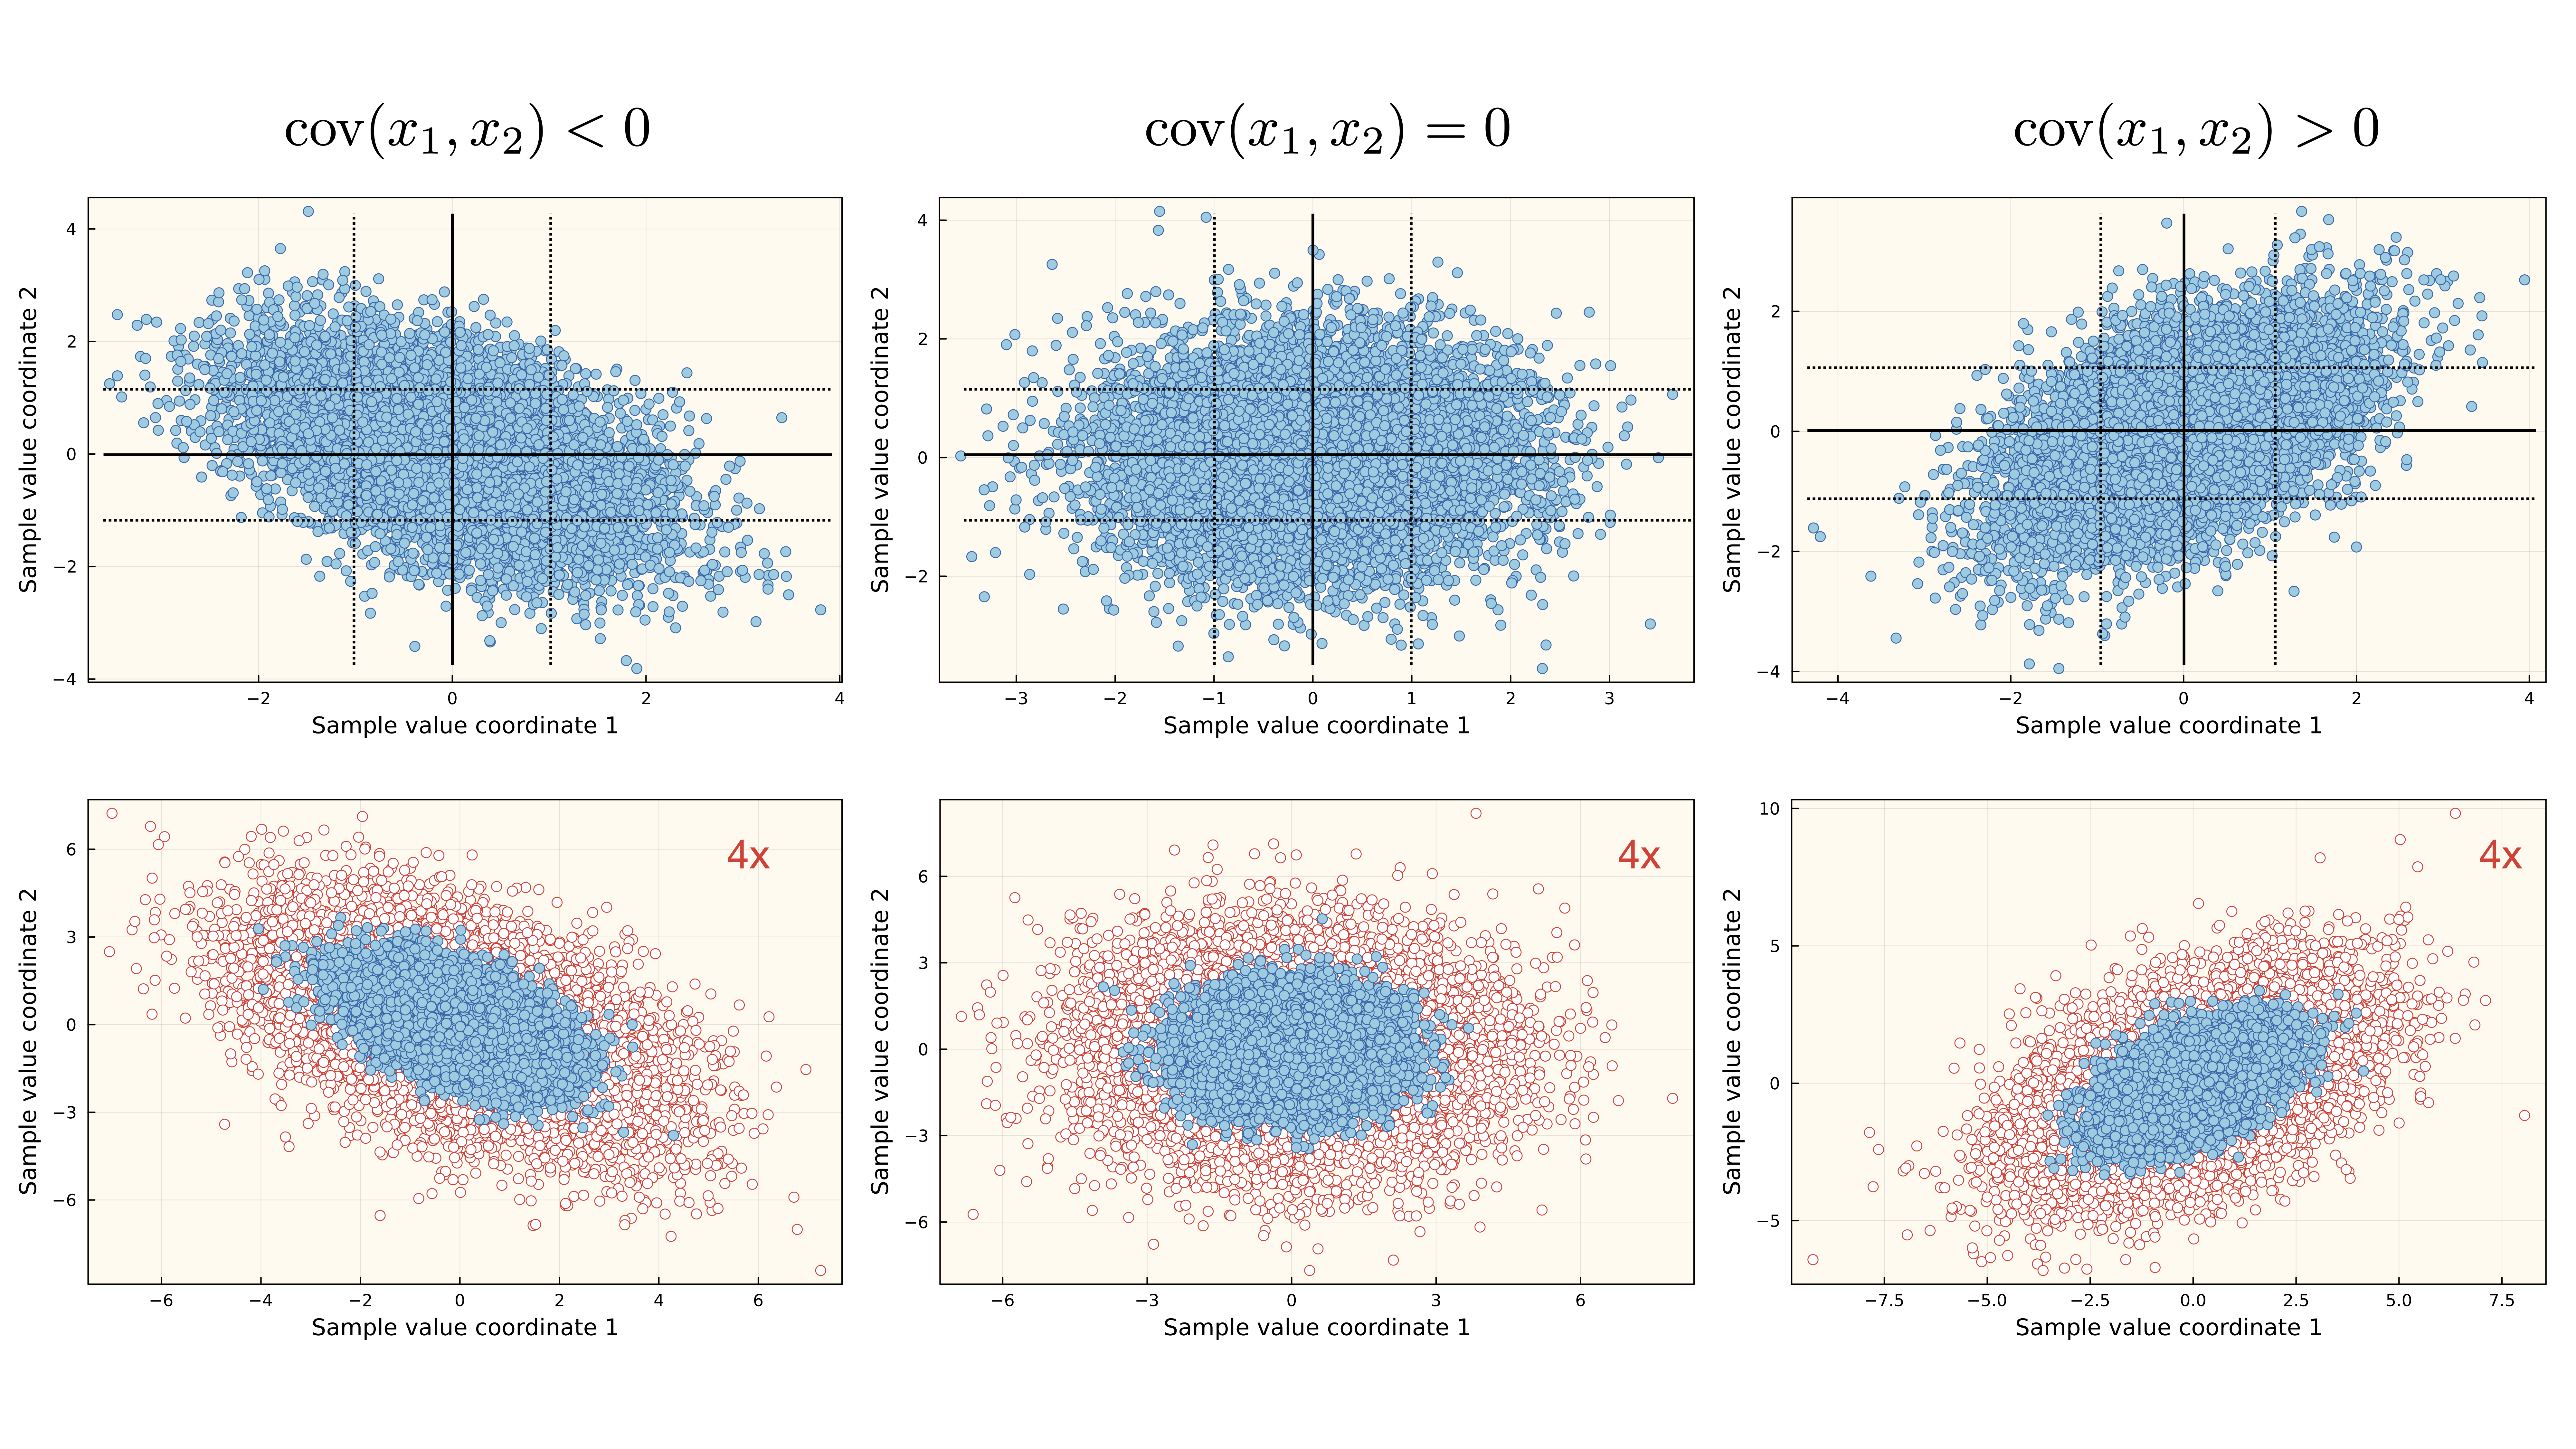
\includegraphics[height=0.68\textheight,keepaspectratio]{../figs/Fig-Cov-Schematic.png}
  \end{center}
  \vspace{-0.3em}
  In the bottom row, each red cloud has four times the blue cloud's covariance
  matrix. Standard deviations double; correlation is unchanged.
\end{frame}

\begin{frame}{Empirical Covariance Matrix}
  Use $N\ge2$ equally spaced periods of growth-rate data for $M$ firms.
  Align the records so every firm's period $k$ covers the same interval.

  \vspace{0.5em}
  Let $g_k^{(i)}$ be firm $i$'s growth rate in period $k$. Its sample mean is:
  \[
    g'_i=\frac{1}{N}\sum_{k=1}^{N}g_k^{(i)}.
  \]
  The empirical growth-rate covariance matrix
  $\Sg\in\mathbb R^{M\times M}$ has entries:
  \[
    \hat\Sigma_{g,ij}=\frac{1}{N-1}\sum_{k=1}^{N}
      \underbrace{\bigl(g_k^{(i)}-g'_i\bigr)}_{\text{deviation for }i}\;
      \underbrace{\bigl(g_k^{(j)}-g'_j\bigr)}_{\text{deviation for }j},
      \qquad i,j\in\mathcal P.
  \]
  Each entry pairs observations from the same period and has units year$^{-2}$.
\end{frame}

\begin{frame}{Interpreting the Covariance Matrix}
  The covariance matrix describes individual growth-rate variability and
  how growth rates move together across firms:

  \vspace{0.5em}
  \begin{itemize}\setlength{\itemsep}{0.8em}
    \item \hilite{Diagonal entries}: $\hat\Sigma_{g,ii}$ is firm $i$'s
      growth-rate variance. Its square root is the growth-rate standard
      deviation $\sigma_g$ for that firm (year$^{-1}$).

      Multiplying by $\sqrt{\Delta t}$ gives the model's volatility estimate:
      \[
        \hat\sigma_i=\sqrt{\Delta t}\,\sqrt{\hat\Sigma_{g,ii}}
        \qquad\text{(year}^{-1/2}\text{).}
      \]
    \item \hilite{Off-diagonal entries}: positive values mean the two growth
      rates tend to deviate from their means in the same direction;
      negative values mean opposite directions.
  \end{itemize}

  \vspace{0.6em}
  Covariance also depends on the scale of each growth-rate series.
  Next, correlation lets us compare relationships on a common scale.
\end{frame}

\begin{frame}{Correlation}
  For firms $i$ and $j$ with positive sample variances, \hilite{correlation}
  divides growth-rate covariance by the product of their standard deviations:
  \[
    \boxed{\rho_{ij}=\frac{\hat\Sigma_{g,ij}}{\sqrt{\hat\Sigma_{g,ii}\,\hat\Sigma_{g,jj}}}\in[-1,1]
    \quad\Longleftrightarrow\quad
    \hat\Sigma_{g,ij}=\rho_{ij}\sqrt{\hat\Sigma_{g,ii}\,\hat\Sigma_{g,jj}}.}
  \]

  This dimensionless ratio lets us compare pairs of firms:

  \vspace{0.4em}
  \begin{itemize}\setlength{\itemsep}{0.6em}
    \item \hilite{Direction and strength}: the sign gives the direction;
      values closer to $-1$ or $1$ indicate a stronger linear relationship.
    \item \hilite{Zero correlation}: no linear relationship in this sample;
      this does not mean the growth rates are independent.
    \item \hilite{Time scaling}: conversions among growth-rate covariance,
      log-return covariance, and covariance rate leave correlation unchanged;
      the common factor cancels.
  \end{itemize}
\end{frame}

\begin{frame}{The Data Matrix and the Sample Covariance}
  Arrange aligned growth rates in $\bG\in\mathbb R^{N\times M}$:
  rows are periods and columns are firms. Compute the covariance matrix
  in two steps:

  \vspace{0.5em}
  \begin{itemize}\setlength{\itemsep}{0.6em}
    \item \hilite{Center each column}: let $\bg'=(g'_1,\ldots,g'_M)^{\top}$
      be the sample-mean vector and $\mathbf 1\in\mathbb R^N$ a vector of ones.
      The outer product repeats these means in every row:
      \[
        \tilde{\bG}=\bG-\mathbf 1\,\bg'^{\top}.
      \]
    \item \hilite{Multiply the centered columns}: the empirical covariance is:
      \[
        \boxed{\Sg=\frac{1}{N-1}\tilde{\bG}^{\top}\tilde{\bG}.}
      \]
  \end{itemize}

  \vspace{0.4em}
  Entry $(i,j)$ is the dot product of centered columns $i$ and $j$, divided
  by $N-1$. This evaluates the earlier covariance formula for every pair at once.
\end{frame}

\begin{frame}{Estimating the Covariance Rate}
  Growth rates and log returns give equivalent estimates of the model's
  covariance rate:

  \vspace{0.4em}
  \begin{itemize}\setlength{\itemsep}{0.65em}
    \item \hilite{From growth-rate data}: the covariance rate and L4b volatility estimates are:
      \[
        \begin{aligned}
          \Ch&=\Delta t\,\Sg
            &&\text{(year}^{-1}\text{)},\\[0.4em]
          \hat\sigma_i&=\sqrt{\hat C_{ii}}
            =\sqrt{\Delta t}\sqrt{\hat\Sigma_{g,ii}}
            &&\text{(year}^{-1/2}\text{)}.
        \end{aligned}
      \]
    \item \hilite{Comparison with log returns}: $\mathbf r=\Delta t\,\bg$ gives:
      \[
        \hat{\boldsymbol\Sigma}_r=(\Delta t)^2\,\Sg=\Delta t\,\Ch
        \qquad\text{(dimensionless).}
      \]
      For daily data with $\Delta t=1/252$ years, both inputs give:
      \[
        \Ch=\frac{\Sg}{252}=252\,\hat{\boldsymbol\Sigma}_r.
      \]
  \end{itemize}
\end{frame}

\begin{frame}{Covariance Matrix Properties}
  The centered-data formula guarantees three properties of our estimate:

  \vspace{0.4em}
  \begin{itemize}\setlength{\itemsep}{0.5em}
    \item \hilite{Elements}: diagonal entries are nonnegative growth-rate
      variances; off-diagonal entries are pairwise covariances.
    \item \hilite{Symmetry}: swapping $i$ and $j$ leaves each product unchanged,
      so $\hat\Sigma_{g,ij}=\hat\Sigma_{g,ji}$.
    \item \hilite{Positive semidefinite}: for any vector $\mathbf v\in\mathbb R^M$,
      the centered-data formula gives:
      \[
        \begin{aligned}
          \mathbf v^{\top}\Sg\mathbf v
          &=\frac{1}{N-1}\mathbf v^{\top}\tilde{\bG}^{\top}\tilde{\bG}\mathbf v\\[0.3em]
          &=\frac{\lVert\tilde{\bG}\mathbf v\rVert_2^2}{N-1}\ge0.
        \end{aligned}
      \]
      This is a squared length divided by $N-1>0$, so every weighted sum
      of growth rates has nonnegative sample variance.
  \end{itemize}

  \vspace{0.4em}
  For $\Delta t>0$, $\Ch=\Delta t\,\Sg$ is also symmetric and positive semidefinite.
\end{frame}

\begin{frame}{Singular Covariance Estimates}
  A positive semidefinite covariance matrix can still be \hilite{singular}:
  it has no inverse. Three points matter when using the estimate:

  \vspace{0.5em}
  \begin{itemize}\setlength{\itemsep}{0.7em}
    \item \hilite{Why it occurs}: centering gives
      $\operatorname{rank}(\tilde{\bG})\le N-1$, so $\Sg$ is singular when
      $M\ge N$. Duplicate series or other exact linear dependencies
      also cause singularity.
    \item \hilite{Choosing a factor}: ordinary Cholesky requires positive
      definiteness. An eigenvalue or singular-value decomposition can still
      provide a covariance factor for simulation when the estimate is singular.
    \item \hilite{Changing the diagonal}: adding a positive value to every
      diagonal entry restores invertibility and increases the modeled variances.
  \end{itemize}
\end{frame}

\begin{frame}{Uncertainty in Covariance Estimates}
  Invertibility does not guarantee a precise or stable estimate.
  Two limitations remain:

  \vspace{0.5em}
  \begin{itemize}\setlength{\itemsep}{0.6em}
    \item \hilite{Sampling error}: we estimate $M(M+1)/2$ distinct variance
      and covariance terms from $N$ periods. When $M$ is large relative to $N$,
      estimates can be noisy and sensitive to the historical window.
    \item \hilite{Changing relationships}: differences between historical
      windows can also reflect changes in how firms' growth rates move together.
  \end{itemize}

  \vspace{0.4em}
  Shrinkage and factor models trade some flexibility for more stable estimates.

  \vspace{0.7em}
  \textbf{\ink{Example:}}
  \href{https://github.com/varnerlab/CHEME-5660-CourseRepository-Fall-2026/blob/main/lectures/week-5/L5a/CHEME-5660-L5a-Example-CovarianceMatrix-Fall-2026.ipynb}{Covariance and Correlation from Data}

  Estimate growth-rate covariance, check the implied volatilities, and compare
  covariance with correlation.
\end{frame}

\begin{frame}{Portfolio Weights}
  Once we can simulate several assets together, we need to specify how much
  to invest in each.

  \vspace{0.6em}
  Let $W_0>0$ be initial wealth in dollars, and let
  $\bw=(w_1,\ldots,w_M)^{\top}$ contain the fractions invested at time zero.

  \vspace{0.6em}
  For a fully invested, long-only portfolio, the weights satisfy:
  \[
    \underbrace{w_i\ge0}_{\text{long only}},\qquad
    \underbrace{\sum_{i=1}^{M}w_i=1}_{\text{fully invested}}.
  \]

  \vspace{0.4em}
  These constraints define the $(M-1)$-dimensional \hilite{simplex}
  $\Delta^{M-1}$: a line segment for two assets and a triangle for three.
\end{frame}

\begin{frame}{Buy-and-Hold Wealth}
  We allow fractional shares and ignore dividends and trading costs.
  Buy $n_i=w_iW_0/S_i(0)$ shares of asset $i$ and hold these share counts fixed.

  \vspace{0.5em}
  Portfolio wealth at time $t$ is:
  \[
    \boxed{W_t=\sum_{i=1}^{M}n_iS_i(t)
      =W_0\sum_{i=1}^{M}w_i\,\frac{S_i(t)}{S_i(0)}.}
  \]

  \vspace{0.4em}
  The fraction of wealth in asset $i$ then becomes:
  \[
    w_i(t)=\frac{n_iS_i(t)}{W_t}.
  \]

  Share counts remain fixed, but weights change as relative prices move.
  Maintaining constant weights requires trading to rebalance the portfolio.
\end{frame}

\begin{frame}{Dirichlet Sampling of the Simplex}
  Draw $\mathbf W\sim\operatorname{Dirichlet}(\boldsymbol\alpha)$, with
  \hilite{concentration parameters} $\boldsymbol\alpha=(\alpha_1,\ldots,\alpha_M)$,
  where $\alpha_i>0$ and $\alpha_0=\sum_{i=1}^{M}\alpha_i$.

  \vspace{0.4em}
  Each draw gives positive weights that sum to one, so the full budget is
  invested. We use a draw as the initial allocation $\bw$. The weight moments are:
  \[
    \begin{gathered}
      \E[W_i]=\frac{\alpha_i}{\alpha_0},\qquad
      \Var(W_i)=\frac{\alpha_i(\alpha_0-\alpha_i)}{\alpha_0^2(\alpha_0+1)},\\[0.5em]
      \Cov(W_i,W_j)=-\frac{\alpha_i\alpha_j}{\alpha_0^2(\alpha_0+1)},\qquad i\ne j.
    \end{gathered}
  \]

  These moments describe the sampled portfolio weights. To evaluate
  portfolio risk, we use the covariance matrix of the firms' growth rates.
\end{frame}

\begin{frame}{How Concentration Shapes the Weights}
  For the three-firm example, changing $\boldsymbol\alpha$ changes how we
  divide the investment:

  \vspace{0.4em}
  \begin{itemize}\setlength{\itemsep}{0.5em}
    \item \hilite{Explore different investment mixes}, $\boldsymbol\alpha=(1,1,1)$:
      no firm is favored; one portfolio might allocate
      70\%, 20\%, and 10\% to the three firms.
    \item \hilite{Concentrate the investment}, $\boldsymbol\alpha=(0.5,0.5,0.5)$:
      favor more uneven allocations, with most money in one or two firms.
    \item \hilite{Stay closer to an equal split}, $\boldsymbol\alpha=(5,5,5)$:
      draws cluster closer to one third of the investment in each firm.
    \item \hilite{Favor the first firm}, $\boldsymbol\alpha=(5,1,1)$:
      it receives about 71\% of the budget on average across draws.
  \end{itemize}

  \vspace{0.5em}
  Both $(1,1,1)$ and $(5,5,5)$ average one third per firm
  \hilite{across many draws}. The larger parameters make
  \hilite{individual portfolios} closer to that equal split.
\end{frame}

\begin{frame}{Approximating Portfolio Growth}
  For an allocation $\bw$ held over one period $\Delta t$, the buy-and-hold
  wealth formula gives the exact portfolio growth rate:
  \[
    \frac{1}{\Delta t}\ln\!\left(\frac{W_{\Delta t}}{W_0}\right)
    =\frac{1}{\Delta t}\ln\!\left(\sum_{i=1}^{M}w_i e^{r_i}\right).
  \]
  Here, $r_i=\ln(S_i(\Delta t)/S_i(0))=g_i\Delta t$ is asset $i$'s log return.

  \vspace{0.5em}
  For small $r_i$, use $e^{r_i}\approx1+r_i$, $\sum_iw_i=1$, and
  $\ln(1+x)\approx x$:
  \[
    \frac{1}{\Delta t}\ln\!\left(\sum_{i=1}^{M}w_i e^{r_i}\right)
    \approx\frac{1}{\Delta t}\sum_{i=1}^{M}w_i r_i
    =\bw^{\top}\bg.
  \]

  We use $g_p=\bw^{\top}\bg$ as a \hilite{linear growth-rate proxy}
  for comparing allocations.
\end{frame}

\begin{frame}{Estimating Portfolio Growth and Risk}
  For each fixed allocation $\bw$, we estimate the mean and variance of
  the linear growth-rate proxy $g_p=\bw^{\top}\bg$ in two steps:

  \vspace{0.5em}
  \textbf{\ink{1. Estimate the inputs from historical growth rates}}
  \begin{itemize}\setlength{\itemsep}{0.4em}
    \item The sample mean vector $\bg^{\prime}$ estimates the model mean
      $\boldsymbol\mu_g$.
    \item The sample covariance matrix $\Sg$ estimates $\Cov(\bg)$.
  \end{itemize}

  \vspace{0.6em}
  \textbf{\ink{2. Evaluate an allocation using its weights}}
  \[
    \begin{aligned}
      \text{Estimated mean growth rate}&=\bw^{\top}\bg^{\prime},\\[0.4em]
      \text{Estimated variance}&=\bw^{\top}\Sg\bw\ge0.
    \end{aligned}
  \]

  The variance accounts for each firm's growth-rate variability and the
  covariances between firms.
\end{frame}

\begin{frame}{From Sampling to Portfolio Choice}
  A Dirichlet draw gives a candidate allocation. We evaluate its estimated
  growth and risk before choosing how to invest:

  \vspace{0.5em}
  \begin{itemize}\setlength{\itemsep}{0.7em}
    \item \hilite{Sampling}: compare many candidate allocations. The
      lowest-variance draw need not minimize variance over all feasible weights.
    \item \hilite{Optimization in L5b}: solve for weights that minimize
      estimated variance, with or without a required mean growth rate.
  \end{itemize}

  \vspace{0.8em}
  \textbf{\ink{Example:}}
  \href{https://github.com/varnerlab/CHEME-5660-CourseRepository-Fall-2026/blob/main/lectures/week-5/L5a/CHEME-5660-L5a-Example-Dirichlet-PortfolioWeights-Fall-2026.ipynb}{Portfolio Weights and the Dirichlet Distribution}

  Explore investment mixes, compare their estimated growth and risk, and
  follow selected buy-and-hold portfolios using the wealth formula.
\end{frame}

% ==== optional advanced material =============================
\begin{frame}{Optional Advanced Material}
  \textbf{\ink{Advanced:}}
  \href{https://github.com/varnerlab/CHEME-5660-CourseRepository-Fall-2026/blob/main/lectures/week-5/L5a/advanced/covariance-estimation/CHEME-5660-L5a-Advanced-CovarianceEstimation-Fall-2026.ipynb}{Sampling Error and Covariance Shrinkage}

  How does estimation error affect portfolio selection? We measure covariance
  error, combine the sample estimate with a simpler matrix, and compare the
  resulting minimum-variance portfolios on later data.

  \vspace{1.0em}
  \textbf{\ink{Advanced:}}
  \href{https://github.com/varnerlab/CHEME-5660-CourseRepository-Fall-2026/blob/main/lectures/week-5/L5a/advanced/rolling-correlation/CHEME-5660-L5a-Advanced-RollingCorrelation-Fall-2026.ipynb}{Rolling Correlations}

  Are the relationships between firms stable over time? Using 2014--2024 data,
  we compare rolling and exponentially weighted correlations and examine
  changes during periods of high market volatility.

  \vspace{0.8em}
  \dimmed{Optional; neither notebook is a prerequisite for L5b.}
\end{frame}

\begin{frame}{Summary}
  We modeled correlated asset prices and examined how the fraction invested
  in each firm affected portfolio growth and risk.

  \vspace{0.7em}
  {\large\textbf{\ink{Key takeaways}}}
  \vspace{0.3em}
  \begin{itemize}\setlength{\itemsep}{0.55em}
    \item \hilite{Correlated asset prices}: We combined independent Wiener
      increments with a loading matrix to model firms whose prices move together.
    \item \hilite{Covariance from data}: We estimated growth-rate covariance
      from historical data and scaled it by the observation interval to obtain
      the model's covariance rate.
    \item \hilite{Portfolio weights}: We used Dirichlet draws to compare
      investment mixes and calculated buy-and-hold wealth from fixed share counts.
  \end{itemize}

  \vspace{0.5em}
  Next time: minimum-variance portfolio optimization and the efficient frontier.
\end{frame}

\transitionframe{Next time: we will use minimum-variance optimization to find
optimal portfolio weights---the weights that minimize estimated variance
under the chosen constraints.}

\end{document}
